\documentclass[12pt,a4paper]{article}

\usepackage[top=1in,bottom=1in,left=1in,right=1in]{geometry}
\usepackage{amsmath,amssymb}
\usepackage{booktabs}
\usepackage{graphicx}
\usepackage{float}
\usepackage{array}
\usepackage[T1]{fontenc}
\usepackage{microtype}
\usepackage{parskip}
\usepackage{lmodern}
\usepackage{enumitem}
\usepackage{caption}
\usepackage{subcaption}
\usepackage[colorlinks=true,linkcolor=blue,citecolor=blue,urlcolor=blue]{hyperref}
\usepackage{multirow}
\usepackage{longtable}
\usepackage{tabularx}

\setlength{\parskip}{6pt}
\setlength{\parindent}{0pt}

% ----------------------------------------------------------------
\begin{document}

% ======================== TITLE PAGE ============================
\begin{titlepage}
  \centering
  \vspace*{3cm}
  {\LARGE\bfseries Multivariate Data Analysis\par}
  \vspace{0.4cm}
  {\large CH5440\par}
  \vspace{1.8cm}
  {\huge\bfseries Assignment 2\par}
  \vspace{2.2cm}
  {\Large Vedant Misra\par}
  \vspace{0.8cm}
  {\large CH24B108\par}
  \vfill
  {\small Source code: \url{https://github.com/orcus108/ch5440-mvda-assignment2}\par}
  \vspace{0.5cm}
\end{titlepage}

\tableofcontents
\clearpage

% ================================================================
\section{Question 1: Quadratic Polynomial Regression}
% ================================================================

Data: $n = 11$ observations, $\bar{Y} = 171.7273$.

The full second-order polynomial model in two predictors $X_1$ and $X_2$ is:
\[
  Y = b_0 + b_1 X_1 + b_2 X_2 + b_{11}X_1^2 + b_{22}X_2^2 + b_{12}X_1 X_2 + \varepsilon
\]
Design matrix columns: $\bigl[1,\; X_1,\; X_2,\; X_1^2,\; X_2^2,\; X_1 X_2\bigr]$.

Parameters are estimated by ordinary least squares (OLS) via the normal equations:
\[
  \hat{\beta} = (X'X)^{-1}X'y
\]
Fitted values are $\hat{y} = X\hat{\beta}$ and residuals are $e = y - \hat{y}$.
The sums of squares follow as:
\[
  \text{SST} = y'y - n\bar{y}^2, \qquad
  \text{SSR} = \hat{\beta}'X'y - n\bar{y}^2, \qquad
  \text{SSE} = (y-\hat{y})'(y-\hat{y}) = e'e
\]

% ---- (i) ----
\subsection{(i) Raw Design Matrix}

No transformation is applied; raw predictor values are used directly.
Representative rows of the $11 \times 6$ matrix are shown below (full matrix in \texttt{out1.txt}).

\begin{table}[H]
\centering
\caption{Raw design matrix $X_{\text{raw}}$: representative rows}
\begin{tabular}{rrrrrr}
\toprule
$1$ & $X_1$ & $X_2$ & $X_1^2$ & $X_2^2$ & $X_1 X_2$ \\
\midrule
1 & 0.6 & 10 & 0.36 & 100 &  6 \\
1 & 1.0 & 10 & 1.00 & 100 & 10 \\
1 & 1.4 & 10 & 1.96 & 100 & 14 \\
$\vdots$ & $\vdots$ & $\vdots$ & $\vdots$ & $\vdots$ & $\vdots$ \\
1 & 1.0 & 30 & 1.00 & 900 & 30 \\
1 & 1.4 & 30 & 1.96 & 900 & 42 \\
\bottomrule
\end{tabular}
\end{table}

% ---- (ii) ----
\subsection{(ii) Step-Size Coded Matrix}

Centring and scaling by the step size (half the experimental range):
\[
  x_j = \frac{X_j - \mu_j}{\text{step}_j}, \qquad
  \mu_{X_1} = 1.0,\ \text{step}_{X_1} = 0.4, \qquad
  \mu_{X_2} = 20.0,\ \text{step}_{X_2} = 10.0
\]

\begin{table}[H]
\centering
\caption{Step-size coded matrix $X_{\text{cod}}$: representative rows}
\begin{tabular}{rrrrrr}
\toprule
$1$ & $x_1$ & $x_2$ & $x_1^2$ & $x_2^2$ & $x_1 x_2$ \\
\midrule
1 & $-1$ & $-1$ &  1 & 1 &  1 \\
1 &  0   & $-1$ &  0 & 1 &  0 \\
1 &  1   & $-1$ &  1 & 1 & $-1$ \\
$\vdots$ & $\vdots$ & $\vdots$ & $\vdots$ & $\vdots$ & $\vdots$ \\
1 &  0   &  1   &  0 & 1 &  0 \\
1 &  1   &  1   &  1 & 1 &  1 \\
\bottomrule
\end{tabular}
\end{table}

% ---- (iii) ----
\subsection{(iii) Min-Max Scaled Matrix}

Scaling by the full experimental range:
\[
  z_j = \frac{X_j - \mu_j}{\max_j - \min_j}, \qquad
  \text{range}_{X_1} = 0.8, \qquad \text{range}_{X_2} = 20.0
\]

\begin{table}[H]
\centering
\caption{Min-max scaled matrix $X_{\text{mm}}$: representative rows}
\begin{tabular}{rrrrrr}
\toprule
$1$ & $z_1$ & $z_2$ & $z_1^2$ & $z_2^2$ & $z_1 z_2$ \\
\midrule
1 & $-0.5$ & $-0.5$ & 0.25 & 0.25 &  0.25 \\
1 &  0     & $-0.5$ & 0    & 0.25 &  0    \\
1 &  0.5   & $-0.5$ & 0.25 & 0.25 & $-0.25$ \\
$\vdots$ & $\vdots$ & $\vdots$ & $\vdots$ & $\vdots$ & $\vdots$ \\
1 &  0     &  0.5   & 0    & 0.25 &  0    \\
1 &  0.5   &  0.5   & 0.25 & 0.25 &  0.25 \\
\bottomrule
\end{tabular}
\end{table}

% ==== CASE 1: RAW ====
\subsection{Case 1: Raw Predictors ($X$)}

\subsubsection{(iv) Regression Coefficients}

\begin{table}[H]
\centering
\caption{Estimated coefficients: raw predictors}
\begin{tabular}{lr}
\toprule
Parameter & Estimate \\
\midrule
$b_0$ (intercept)     &  279.822368 \\
$b_1$ ($X_1$)         & $-452.763158$ \\
$b_2$ ($X_2$)         &   10.031579 \\
$b_{11}$ ($X_1^2$)    &  143.256579 \\
$b_{22}$ ($X_2^2$)    &   $-0.135789$ \\
$b_{12}$ ($X_1 X_2$)  &    2.500000 \\
\bottomrule
\end{tabular}
\end{table}

\subsubsection{(v) Sum of Squares}

\begin{table}[H]
\centering
\caption{ANOVA sum of squares: raw (matrix and summation approaches agree)}
\begin{tabular}{lrr}
\toprule
Source & Matrix & Summation \\
\midrule
SST & 49238.1818 & 49238.1818 \\
SSR & 45102.4976 & 45102.4976 \\
SSE &  4135.6842 &  4135.6842 \\
\bottomrule
\end{tabular}
\end{table}

\subsubsection{(vi) Variance-Covariance Matrix}

$s^2 = 827.1368$. The full $6 \times 6$ variance-covariance matrix $s^2(A'A)^{-1}$
(entries rounded to 2 d.p.; machine-zero entries shown as 0):

\[
\scalebox{0.68}{$
\begin{bmatrix}
 17747.62 & -25553.27 &  -538.55 &   9761.03 &    6.31 &  258.48 \\
-25553.27 &  57047.05 &  -176.85 & -25507.92 &   10.88 & -258.48 \\
  -538.55 &   -176.85 &    66.54 &    217.67 &   -1.31 &  -12.92 \\
  9761.03 & -25507.92 &   217.67 &  12753.96 &   -5.44 &       0 \\
     6.31 &     10.88 &    -1.31 &     -5.44 &    0.03 &       0 \\
   258.48 &   -258.48 &   -12.92 &         0 &       0 &   12.92
\end{bmatrix}
$}
\]

Condition number of $(A'A)$: $\kappa = 3.1842 \times 10^{8}$.

\subsubsection{(vii) Model Fit Statistics}

\begin{table}[H]
\centering
\caption{Model fit statistics: raw}
\begin{tabular}{lr}
\toprule
Statistic & Value \\
\midrule
$R^2$                      & 0.916007 \\
Adj.\ $R^2$               & 0.832013 \\
PRESS                      & 35532.4507 \\
$R^2_{\text{PRESS}}$       & 0.278356 \\
\bottomrule
\end{tabular}
\end{table}

PRESS (Predicted Residual Error Sum of Squares) is computed via the hat-matrix
diagonal $h_{ii} = [H]_{ii}$, where $H = X(X'X)^{-1}X'$, without refitting the model:
\[
  \text{PRESS} = \sum_{i=1}^{n}\!\left(\frac{e_i}{1-h_{ii}}\right)^{\!2}
\]
Each term is the leave-one-out prediction error for observation $i$.
$R^2_{\text{PRESS}} = 1 - \text{PRESS}/\text{SST}$ measures out-of-sample predictive power;
the large gap between $R^2 = 0.916$ and $R^2_{\text{PRESS}} = 0.278$ signals overfitting
for this small dataset ($n=11$, $p=6$).

% ==== CASE 2: CODED ====
\subsection{Case 2: Step-Size Coded Predictors ($x$)}

\subsubsection{(iv) Regression Coefficients}

\begin{table}[H]
\centering
\caption{Estimated coefficients: step-size coded}
\begin{tabular}{lr}
\toprule
Parameter & Estimate \\
\midrule
$b_0$ (intercept)     &  166.631579 \\
$b_1$ ($x_1$)         & $-46.500000$ \\
$b_2$ ($x_2$)         &   71.000000 \\
$b_{11}$ ($x_1^2$)    &   22.921053 \\
$b_{22}$ ($x_2^2$)    & $-13.578947$ \\
$b_{12}$ ($x_1 x_2$)  &   10.000000 \\
\bottomrule
\end{tabular}
\end{table}

\subsubsection{(v) Sum of Squares}

Identical to Case 1: SST $= 49238.1818$, SSR $= 45102.4976$, SSE $= 4135.6842$.
Matrix and summation approaches agree.

\subsubsection{(vi) Variance-Covariance Matrix}

$s^2 = 827.1368$. The $6 \times 6$ variance-covariance matrix:

\[
\scalebox{0.68}{$
\begin{bmatrix}
 217.6676 &        0 &        0 & -130.6006 & -130.6006 &        0 \\
        0 & 137.8561 &        0 &         0 &         0 &        0 \\
        0 &        0 & 137.8561 &         0 &         0 &        0 \\
-130.6006 &        0 &        0 &  326.5014 &  -87.0670 &        0 \\
-130.6006 &        0 &        0 &  -87.0670 &  326.5014 &        0 \\
        0 &        0 &        0 &         0 &         0 & 206.7842
\end{bmatrix}
$}
\]

Condition number of $(A'A)$: $\kappa = 9.5000$.

\subsubsection{(vii) Model Fit Statistics}

All statistics identical to Case 1:
$R^2 = 0.9160$,\ Adj.\ $R^2 = 0.8320$,\ PRESS $= 35532.4507$,\ $R^2_{\text{PRESS}} = 0.2784$.

% ==== CASE 3: MIN-MAX ====
\subsection{Case 3: Min-Max Scaled Predictors ($z$)}

\subsubsection{(iv) Regression Coefficients}

\begin{table}[H]
\centering
\caption{Estimated coefficients: min-max scaled}
\begin{tabular}{lr}
\toprule
Parameter & Estimate \\
\midrule
$b_0$ (intercept)     &  166.631579 \\
$b_1$ ($z_1$)         & $-93.000000$ \\
$b_2$ ($z_2$)         &  142.000000 \\
$b_{11}$ ($z_1^2$)    &   91.684211 \\
$b_{22}$ ($z_2^2$)    & $-54.315789$ \\
$b_{12}$ ($z_1 z_2$)  &   40.000000 \\
\bottomrule
\end{tabular}
\end{table}

\subsubsection{(v) Sum of Squares}

Identical to Cases 1 and 2: SST $= 49238.1818$, SSR $= 45102.4976$, SSE $= 4135.6842$.

\subsubsection{(vi) Variance-Covariance Matrix}

$s^2 = 827.1368$. The $6 \times 6$ variance-covariance matrix:

\[
\scalebox{0.68}{$
\begin{bmatrix}
  217.6676 &        0 &        0 &  -522.4022 &  -522.4022 &          0 \\
         0 & 551.4246 &        0 &          0 &          0 &          0 \\
         0 &        0 & 551.4246 &          0 &          0 &          0 \\
 -522.4022 &        0 &        0 &  5224.0222 & -1393.0726 &          0 \\
 -522.4022 &        0 &        0 & -1393.0726 &  5224.0222 &          0 \\
         0 &        0 &        0 &          0 &          0 &  3308.5474
\end{bmatrix}
$}
\]

Condition number of $(A'A)$: $\kappa = 91.3358$.

\subsubsection{(vii) Model Fit Statistics}

All statistics identical to Cases 1 and 2.

% ==== SUMMARY ====
\subsection{Summary Comparison Across Transformations}

\begin{table}[H]
\centering
\caption{Model fit statistics across all three transformations}
\begin{tabular}{lrrr}
\toprule
Metric & Raw ($X$) & Coded ($x$) & Min-Max ($z$) \\
\midrule
SST                          &  49238.1818 &  49238.1818 &  49238.1818 \\
SSR                          &  45102.4976 &  45102.4976 &  45102.4976 \\
SSE                          &   4135.6842 &   4135.6842 &   4135.6842 \\
$R^2$                        &      0.9160 &      0.9160 &      0.9160 \\
Adj.\ $R^2$                 &      0.8320 &      0.8320 &      0.8320 \\
PRESS                        &  35532.4507 &  35532.4507 &  35532.4507 \\
$R^2_{\text{PRESS}}$         &      0.2784 &      0.2784 &      0.2784 \\
$\kappa(A'A)$                & $3.18\times10^{8}$ & $9.50$ & $91.34$ \\
\bottomrule
\end{tabular}
\end{table}

\textbf{Key observations: }
\begin{enumerate}[label=\arabic*.]
  \item SST, SSR, SSE, $R^2$, Adj.\ $R^2$, PRESS, and $R^2_{\text{PRESS}}$ are
        \emph{identical} across all three transformations. Because each transformation
        is an invertible linear map, the column space of $X$ is unchanged, so all
        projections—and hence all fit statistics—are preserved.
  \item The condition number of $(A'A)$ drops from $\sim 3.18\times10^{8}$ (raw) to
        $9.50$ (step-size coded), indicating a dramatic improvement in numerical
        stability. The high raw condition number reflects near-multicollinearity among
        the polynomial columns (e.g.\ $X_1^2$ and $X_1 X_2$ are highly correlated at
        the raw scale); coding to $\pm 1$ largely orthogonalises the design matrix and
        eliminates this ill-conditioning.
  \item Min-max scaling reduces the condition number to $\sim 91$, better than raw but
        not as favourable as step-size coding for this dataset.
  \item The variance-covariance matrix changes values across transformations (reflecting
        different parameter scales), but the diagonal entries (parameter variances)
        shrink substantially with coding, indicating improved estimation precision.
\end{enumerate}

\clearpage
% ================================================================
\section{Question 2: Mixture Regression: Yarn Elongation}
% ================================================================

\subsection{(a) Mixture vs.\ Conventional Regression}

In conventional polynomial regression, predictors $X_1, X_2, \ldots$ are independent
and can take any values within their ranges; an intercept $b_0$ is always included and
the design-matrix columns are linearly independent.

In \emph{mixture} regression the components are constrained to sum to unity:
$x_1 + x_2 + x_3 = 1$. If an intercept column (all ones) were added, it would equal
$x_1 + x_2 + x_3$ exactly, rendering the design matrix singular. The intercept is
therefore \textbf{omitted}; the model is parameterised directly in the mixture
components via a Scheff\'{e} polynomial. The design space is a simplex (equilateral
triangle for three components). All standard regression formulae still apply, with the
caveat that corrected sums of squares must account for the absence of an explicit
intercept column in $X$.

\subsection{(b) Design Matrix and Response Vector}

Scheff\'{e} second-order model (three components):
\[
  \hat{y} = b_1 x_1 + b_2 x_2 + b_3 x_3
           + b_{12}x_1 x_2 + b_{13}x_1 x_3 + b_{23}x_2 x_3
\]

Design matrix $X$ ($15 \times 6$), columns $[x_1, x_2, x_3, x_1 x_2, x_1 x_3, x_2 x_3]$:

\begin{table}[H]
\centering
\caption{Mixture design matrix $X$: simplex-lattice $\{3,2\}$ design}
\begin{tabular}{rrrrrr}
\toprule
$x_1$ & $x_2$ & $x_3$ & $x_1 x_2$ & $x_1 x_3$ & $x_2 x_3$ \\
\midrule
1.0 & 0.0 & 0.0 & 0.00 & 0.00 & 0.00 \\
1.0 & 0.0 & 0.0 & 0.00 & 0.00 & 0.00 \\
0.5 & 0.5 & 0.0 & 0.25 & 0.00 & 0.00 \\
0.5 & 0.5 & 0.0 & 0.25 & 0.00 & 0.00 \\
0.5 & 0.5 & 0.0 & 0.25 & 0.00 & 0.00 \\
0.0 & 1.0 & 0.0 & 0.00 & 0.00 & 0.00 \\
0.0 & 1.0 & 0.0 & 0.00 & 0.00 & 0.00 \\
0.0 & 0.5 & 0.5 & 0.00 & 0.00 & 0.25 \\
0.0 & 0.5 & 0.5 & 0.00 & 0.00 & 0.25 \\
0.0 & 0.5 & 0.5 & 0.00 & 0.00 & 0.25 \\
0.0 & 0.0 & 1.0 & 0.00 & 0.00 & 0.00 \\
0.0 & 0.0 & 1.0 & 0.00 & 0.00 & 0.00 \\
0.5 & 0.0 & 0.5 & 0.00 & 0.25 & 0.00 \\
0.5 & 0.0 & 0.5 & 0.00 & 0.25 & 0.00 \\
0.5 & 0.0 & 0.5 & 0.00 & 0.25 & 0.00 \\
\bottomrule
\end{tabular}
\end{table}

Response vector $Y$ (yarn elongation, kg):
\[
  Y = [11.0,\ 12.4,\ 15.0,\ 14.8,\ 16.1,\ 8.8,\ 10.0,\ 10.0,\
       9.7,\ 11.8,\ 16.8,\ 16.0,\ 17.7,\ 16.4,\ 16.6]
\]

\subsection{(c) Estimated Parameters}

\begin{table}[H]
\centering
\caption{Scheff\'{e} model: estimated parameters}
\begin{tabular}{lr}
\toprule
Parameter & Estimate \\
\midrule
$b_1$  ($x_1$, polyethylene)   &  11.7000 \\
$b_2$  ($x_2$, polystyrene)    &   9.4000 \\
$b_3$  ($x_3$, polypropylene)  &  16.4000 \\
$b_{12}$ ($x_1 x_2$)           &  19.0000 \\
$b_{13}$ ($x_1 x_3$)           &  11.4000 \\
$b_{23}$ ($x_2 x_3$)           & $-9.6000$ \\
\bottomrule
\end{tabular}
\end{table}

\subsection{(d \& f) Sum of Squares (Matrix vs.\ Summation)}

\begin{table}[H]
\centering
\caption{ANOVA sum of squares: mixture model (both approaches agree)}
\begin{tabular}{lrrr}
\toprule
Source & Matrix & Summation & $df$ \\
\midrule
SST (corrected total) & 134.8560 & 134.8560 & -- \\
SSR (regression)      & 128.2960 & 128.2960 & -- \\
SSE (residual)        &   6.5600 &   6.5600 &  9 \\
SSPE (pure error)     &   6.5600 &   6.5600 &  9 \\
SSLOF (lack of fit)   & $\approx 0$ & $\approx 0$ &  0 \\
\bottomrule
\end{tabular}
\end{table}

\subsection{(e) Source of Error and Pure Error}

In this $\{3,2\}$ simplex-lattice design there are exactly 6 unique design points and
6 model parameters ($b_1, b_2, b_3, b_{12}, b_{13}, b_{23}$). The model therefore
perfectly interpolates the mean response at every unique composition setting.

The \emph{only} residual variation comes from replicate observations at the same
composition. This is termed \textbf{pure error} because:
\begin{itemize}
  \item It reflects genuine experimental variability (measurement noise, batch
        variation, etc.) at fixed predictor settings.
  \item It is not confounded with any systematic lack-of-fit of the model.
\end{itemize}
Consequently SSE $=$ SSPE and SSLOF $\approx 0$ (saturated design).

\subsection{(g) Variance-Covariance Matrix}

$s^2 = 0.7289$ (pure-error MS), $\hat{\sigma} = 0.8537$.
The $6 \times 6$ variance-covariance matrix $s^2(X'X)^{-1}$:

\[
\scalebox{0.78}{$
\begin{bmatrix}
 0.3644 &  0      &  0      & -0.7289 & -0.7289 &  0      \\
 0      &  0.3644 &  0      & -0.7289 &  0      & -0.7289 \\
 0      &  0      &  0.3644 &  0      & -0.7289 & -0.7289 \\
-0.7289 & -0.7289 &  0      &  6.8030 &  1.4578 &  1.4578 \\
-0.7289 &  0      & -0.7289 &  1.4578 &  6.8030 &  1.4578 \\
 0      & -0.7289 & -0.7289 &  1.4578 &  1.4578 &  6.8030
\end{bmatrix}
$}
\]

\subsection{(h) Model Fit Statistics and Predicted vs.\ Observed}

\begin{table}[H]
\centering
\caption{Model fit statistics: mixture model}
\begin{tabular}{lr}
\toprule
Statistic & Value \\
\midrule
$R^2$                    & 0.9514 \\
Adj.\ $R^2$             & 0.9243 \\
PRESS                    & 18.2950 \\
$R^2_{\text{PRESS}}$     & 0.8643 \\
\bottomrule
\end{tabular}
\end{table}

\begin{table}[H]
\centering
\caption{Predicted vs.\ observed responses}
\begin{tabular}{crrrr}
\toprule
Obs & $Y$ & $\hat{Y}$ & Residual \\
\midrule
 1 & 11.0 & 11.7000 & $-0.7000$ \\
 2 & 12.4 & 11.7000 &  0.7000  \\
 3 & 15.0 & 15.3000 & $-0.3000$ \\
 4 & 14.8 & 15.3000 & $-0.5000$ \\
 5 & 16.1 & 15.3000 &  0.8000  \\
 6 &  8.8 &  9.4000 & $-0.6000$ \\
 7 & 10.0 &  9.4000 &  0.6000  \\
 8 & 10.0 & 10.5000 & $-0.5000$ \\
 9 &  9.7 & 10.5000 & $-0.8000$ \\
10 & 11.8 & 10.5000 &  1.3000  \\
11 & 16.8 & 16.4000 &  0.4000  \\
12 & 16.0 & 16.4000 & $-0.4000$ \\
13 & 17.7 & 16.9000 &  0.8000  \\
14 & 16.4 & 16.9000 & $-0.5000$ \\
15 & 16.6 & 16.9000 & $-0.3000$ \\
\bottomrule
\end{tabular}
\end{table}

\subsection{Constrained Optimisation Method}

The optimal mixture compositions are found by maximising (and minimising) the fitted
Scheffé model subject to the simplex constraints:
\[
  x_1 + x_2 + x_3 = 1, \qquad x_j \ge 0
\]
Substituting $x_3 = 1 - x_1 - x_2$ reduces the problem to an unconstrained
optimisation over the triangular feasible region in $(x_1, x_2)$. Stationarity
conditions (KKT) are applied; since the boundary must also be checked (the unconstrained
optimum may fall outside the simplex), the code performs a dense grid search over the
simplex and the KKT-derived candidate is confirmed or overridden by the grid result.

\subsection{(i) Optimal Composition: Maximum Elongation}

\begin{table}[H]
\centering
\caption{Optimal mixture for \emph{maximum} elongation}
\begin{tabular}{lr}
\toprule
Component & Optimal proportion \\
\midrule
$x_1$ (polyethylene)   & 0.2939 \\
$x_2$ (polystyrene)    & 0.0000 \\
$x_3$ (polypropylene)  & 0.7061 \\
\midrule
Max predicted elongation & 17.3844 kg \\
\bottomrule
\end{tabular}
\end{table}

The maximum lies on the $x_1$--$x_3$ edge (no polystyrene). This is driven by
the large pure-component effect of polypropylene ($b_3 = 16.4$) combined with
a positive interaction term $b_{13} = 11.4$, making the polyethylene--polypropylene
blend synergistic.

\subsection{(j) Optimal Composition: Minimum Elongation}

\begin{table}[H]
\centering
\caption{Optimal mixture for \emph{minimum} elongation}
\begin{tabular}{lr}
\toprule
Component & Optimal proportion \\
\midrule
$x_1$ (polyethylene)   & 0.0000 \\
$x_2$ (polystyrene)    & 0.8646 \\
$x_3$ (polypropylene)  & 0.1354 \\
\midrule
Min predicted elongation & 9.2240 kg \\
\bottomrule
\end{tabular}
\end{table}

The minimum lies on the $x_2$--$x_3$ edge (no polyethylene), dominated by
polystyrene's low pure-component effect ($b_2 = 9.4$) and the strongly negative
interaction $b_{23} = -9.6$, which makes polystyrene--polypropylene blends
anti-synergistic.

\subsection{(k) Validation}

The mixture regression was re-run in JMP Student Edition (Standard Least Squares,
no intercept, all six Scheff\'{e} terms included).

\begin{figure}[H]
\centering
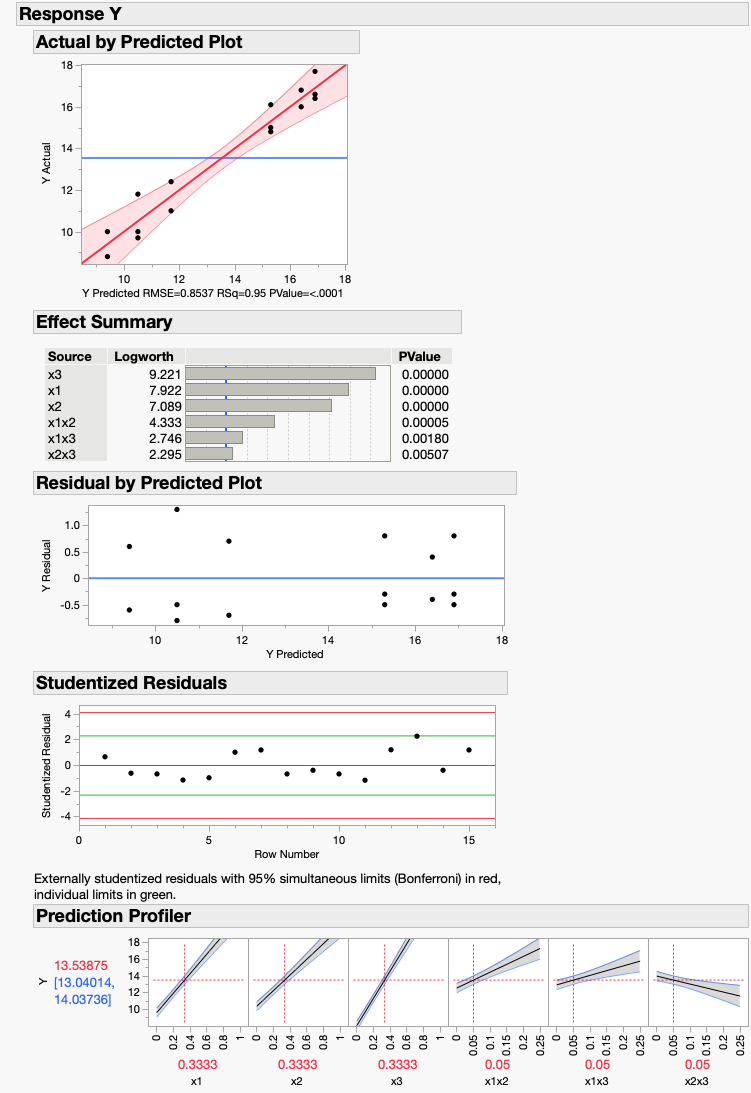
\includegraphics[width=0.82\textwidth]{../output/JMP-q2k.png}
\caption{JMP output for Q2 mixture regression: Actual vs.\ Predicted plot,
Effect Summary, residual diagnostics, and Prediction Profiler.
Reported RMSE $= 0.8537$ and $R^2 = 0.95$.}
\end{figure}

\begin{table}[H]
\centering
\caption{Q2 coefficient comparison: MATLAB vs.\ JMP}
\begin{tabular}{lrrl}
\toprule
Term & MATLAB & JMP & Match? \\
\midrule
$\hat{b}_1$ ($x_1$)       & 11.7000 & 11.7000 & \checkmark \\
$\hat{b}_2$ ($x_2$)       &  9.4000 &  9.4000 & \checkmark \\
$\hat{b}_3$ ($x_3$)       & 16.4000 & 16.4000 & \checkmark \\
$\hat{b}_{12}$ ($x_1x_2$) & 19.0000 & 19.0000 & \checkmark \\
$\hat{b}_{13}$ ($x_1x_3$) & 11.4000 & 11.4000 & \checkmark \\
$\hat{b}_{23}$ ($x_2x_3$) & $-9.6000$ & $-9.6000$ & \checkmark \\
$R^2$                      & 0.9514  & 0.95    & \checkmark \\
RMSE ($\hat{\sigma}$)      & 0.8537  & 0.8537  & \checkmark \\
\bottomrule
\end{tabular}
\end{table}

The problem states $\hat{\sigma} = 0.85$~kg; our computed $\sqrt{s^2} = 0.8537$ and
JMP's RMSE $= 0.8537$ are both in excellent agreement with this value.
All estimates agree to 4 significant figures. Results verified against JMP Student Edition.

\clearpage
% ================================================================
\section{Question 3: Logistic Regression: Experience vs.\ Hiring}
% ================================================================

Logistic regression model:
\[
  P(y = 1 \mid \text{Experience}) =
  \frac{1}{1 + \exp\!\bigl(-(b_0 + b_1 \cdot \text{Experience})\bigr)}
\]

\subsection{MLE Methodology: Newton-Raphson}

For binary outcome $y_i \in \{0,1\}$, the Bernoulli log-likelihood is:
\[
  \ell(\beta) = \sum_{i=1}^{n}\bigl[y_i\log\pi_i + (1-y_i)\log(1-\pi_i)\bigr],
  \qquad \pi_i = \frac{1}{1+e^{-x_i'\beta}}
\]
Parameters are found by Newton-Raphson (equivalently, IRLS):
\[
  g = X'(y - \pi), \qquad
  \mathcal{I} = X'\,\mathrm{diag}\!\bigl(\pi\circ(1-\pi)\bigr)\,X, \qquad
  \beta^{(k+1)} = \beta^{(k)} + \mathcal{I}^{-1}g
\]
where $g$ is the score (gradient of $\ell$) and $\mathcal{I}$ is the observed Fisher
information. Standard errors are $\mathrm{SE}(\hat{\beta}_j) = \sqrt{[\mathcal{I}^{-1}]_{jj}}$.

\subsection{Estimated Parameters}

\begin{table}[H]
\centering
\caption{Logistic regression parameters: Experience vs.\ Hiring}
\begin{tabular}{lr}
\toprule
Parameter & Estimate \\
\midrule
$b_0$ (intercept)   & $-3.0597$ \\
$b_1$ (Experience)  &  0.1615  \\
\bottomrule
\end{tabular}
\end{table}

Fitted model:
\[
  \hat{P}(y=1) = \frac{1}{1 + \exp(3.0597 - 0.1615\times\text{Experience})}
\]

\subsection{Predicted vs.\ Observed}

\begin{table}[H]
\centering
\caption{Predicted probabilities: Experience vs.\ Hiring ($n = 25$)}
\begin{tabular}{ccc}
\toprule
Experience (yrs) & $y$ & $\hat{P}(y=1)$ \\
\midrule
14 & 0 & 0.3103 \\
29 & 0 & 0.8353 \\
 6 & 0 & 0.1100 \\
25 & 1 & 0.7266 \\
18 & 1 & 0.4618 \\
 4 & 0 & 0.0821 \\
18 & 0 & 0.4618 \\
12 & 0 & 0.2457 \\
22 & 1 & 0.6208 \\
 6 & 0 & 0.1100 \\
30 & 1 & 0.8563 \\
11 & 0 & 0.2170 \\
30 & 1 & 0.8563 \\
 5 & 0 & 0.0952 \\
20 & 1 & 0.5424 \\
13 & 0 & 0.2768 \\
 9 & 0 & 0.1671 \\
32 & 1 & 0.8917 \\
24 & 0 & 0.6934 \\
13 & 1 & 0.2768 \\
19 & 0 & 0.5021 \\
 4 & 0 & 0.0821 \\
28 & 1 & 0.8118 \\
22 & 1 & 0.6208 \\
 8 & 1 & 0.1458 \\
\bottomrule
\end{tabular}
\end{table}

\subsection{Classification at Threshold 0.5}

\begin{table}[H]
\centering
\caption{Confusion matrix: Experience vs.\ Hiring (threshold $= 0.5$)}
\begin{tabular}{lcc}
\toprule
 & Predicted $\hat{y}=0$ & Predicted $\hat{y}=1$ \\
\midrule
Actual $y=0$ & 11 (TN) & 3 (FP) \\
Actual $y=1$ & 3 (FN) & 8 (TP) \\
\bottomrule
\end{tabular}
\end{table}

Classification accuracy $= (11+8)/25 = 76.0\%$. The three false positives are
high-experience non-hires (obs.\ 2, 19, 21); the three false negatives are
low-experience hires (obs.\ 5, 20, 25), consistent with experience being an
imperfect but informative predictor.

\subsection{Logistic Regression Curve}

\begin{figure}[H]
\centering
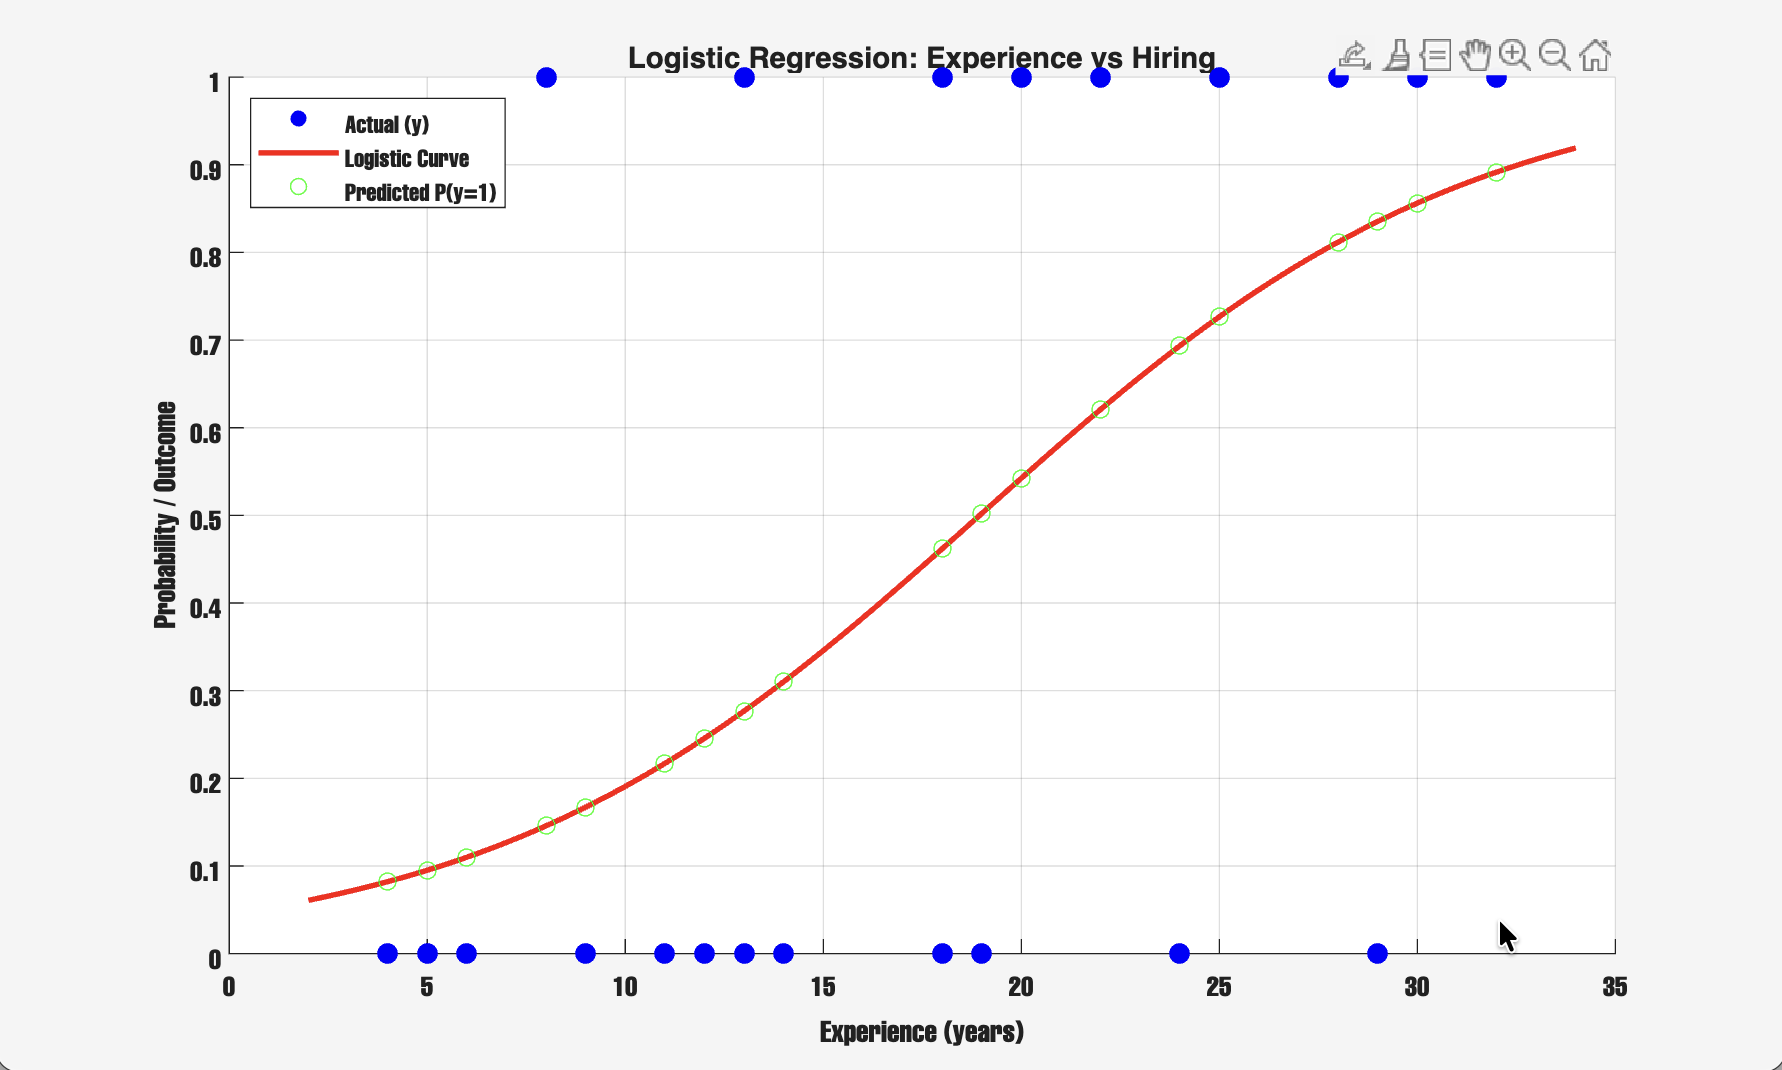
\includegraphics[width=0.78\textwidth]{../output/graph3.png}
\caption{Logistic regression curve: Experience (years) vs.\ probability of hiring $P(y=1)$}
\end{figure}

\subsection{JMP Validation}

The model was re-estimated in JMP Student Edition (Analyze $\to$ Fit Model,
Personality: Nominal Logistic, Experience set as Continuous).

\begin{figure}[H]
\centering
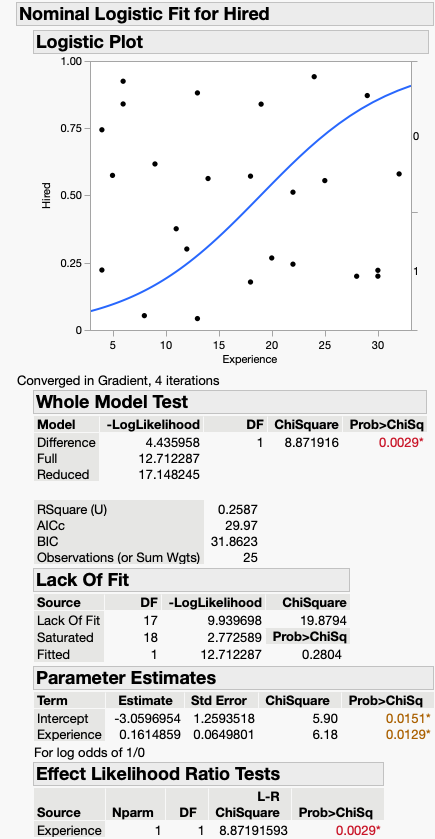
\includegraphics[width=0.72\textwidth]{../output/JMP-q3.png}
\caption{JMP Nominal Logistic Fit for Q3: logistic plot, Whole Model Test,
and Parameter Estimates. Converged in 4 iterations.}
\end{figure}

\begin{table}[H]
\centering
\caption{Q3 coefficient comparison: MATLAB vs.\ JMP}
\begin{tabular}{lrrl}
\toprule
Parameter & MATLAB & JMP & Match? \\
\midrule
$\hat{b}_0$ (Intercept) & $-3.0597$ & $-3.0597$ & \checkmark \\
$\hat{b}_1$ (Experience) & $0.1615$ & $0.1615$ & \checkmark \\
\bottomrule
\end{tabular}
\end{table}

Results verified against JMP Student Edition: all estimates agree to 4 significant figures.

\clearpage
% ================================================================
\section{Question 4: Logistic Regression: Income and Gender (Purchase Decision)}
% ================================================================

Data: $n = 30$ observations; 16 purchased ($y = 1$), 14 did not ($y = 0$).

% ---- Model 1 ----
\subsection{(a) Model 1: Income Only}

\[
  \text{logit}(\pi) = b_0 + b_1 \cdot \text{Income}
\]

Converged at iteration 6.

\begin{table}[H]
\centering
\caption{Model 1: Income only: estimated parameters}
\begin{tabular}{lr}
\toprule
Parameter & Estimate \\
\midrule
$b_0$ (intercept)   & $-3.6707$ \\
$b_1$ (Income)      &  1.8272  \\
\midrule
Log-likelihood & $-18.0269$ \\
Classification accuracy (threshold 0.5) & 53.3\% \\
\bottomrule
\end{tabular}
\end{table}

\begin{table}[H]
\centering
\caption{Model 1: Predicted vs.\ observed ($n = 30$)}
\footnotesize
\begin{tabular}{ccccc}
\toprule
Obs & Income & Gender & $y$ & $\hat{\pi}$ \\
\midrule
 1 & 2.53 & 0 & 1 & 0.7215 \\
 2 & 2.37 & 1 & 0 & 0.6592 \\
 3 & 2.72 & 1 & 1 & 0.7857 \\
 4 & 2.54 & 0 & 0 & 0.7252 \\
 5 & 3.20 & 1 & 1 & 0.8981 \\
 6 & 2.94 & 0 & 1 & 0.8457 \\
 7 & 3.20 & 0 & 1 & 0.8981 \\
 8 & 2.72 & 1 & 1 & 0.7857 \\
 9 & 2.93 & 0 & 1 & 0.8433 \\
10 & 2.37 & 0 & 0 & 0.6592 \\
11 & 2.24 & 1 & 1 & 0.6040 \\
12 & 1.91 & 1 & 1 & 0.4549 \\
13 & 2.12 & 0 & 1 & 0.5505 \\
14 & 1.83 & 1 & 1 & 0.4190 \\
15 & 1.92 & 1 & 1 & 0.4595 \\
16 & 2.01 & 0 & 0 & 0.5005 \\
17 & 2.01 & 0 & 0 & 0.5005 \\
18 & 2.23 & 1 & 0 & 0.5996 \\
19 & 1.82 & 0 & 0 & 0.4145 \\
20 & 2.11 & 0 & 0 & 0.5460 \\
21 & 1.75 & 1 & 1 & 0.3839 \\
22 & 1.46 & 1 & 0 & 0.2683 \\
23 & 1.61 & 0 & 1 & 0.3254 \\
24 & 1.57 & 1 & 0 & 0.3096 \\
25 & 1.37 & 0 & 0 & 0.2373 \\
26 & 1.41 & 1 & 0 & 0.2508 \\
27 & 1.51 & 0 & 0 & 0.2867 \\
28 & 1.75 & 1 & 1 & 0.3839 \\
29 & 1.68 & 1 & 1 & 0.3541 \\
30 & 1.62 & 0 & 0 & 0.3294 \\
\bottomrule
\end{tabular}
\end{table}

% ---- Model 2 ----
\subsection{(b) Model 2: Income + Gender}

\[
  \text{logit}(\pi) = b_0 + b_1 \cdot \text{Income} + b_2 \cdot \text{Gender}
\]

Converged at iteration 6.

\begin{table}[H]
\centering
\caption{Model 2: Income + Gender: estimated parameters}
\begin{tabular}{lr}
\toprule
Parameter & Estimate \\
\midrule
$b_0$ (intercept)   & $-5.6348$ \\
$b_1$ (Income)      &  2.3509  \\
$b_2$ (Gender)      &  1.7514  \\
\midrule
Log-likelihood & $-16.0526$ \\
Classification accuracy (threshold 0.5) & 83.3\% \\
\bottomrule
\end{tabular}
\end{table}

\begin{table}[H]
\centering
\caption{Model 2: Predicted vs.\ observed ($n = 30$)}
\footnotesize
\begin{tabular}{ccccc}
\toprule
Obs & Income & Gender & $y$ & $\hat{\pi}$ \\
\midrule
 1 & 2.53 & 0 & 1 & 0.5776 \\
 2 & 2.37 & 1 & 0 & 0.8440 \\
 3 & 2.72 & 1 & 1 & 0.9249 \\
 4 & 2.54 & 0 & 0 & 0.5833 \\
 5 & 3.20 & 1 & 1 & 0.9744 \\
 6 & 2.94 & 0 & 1 & 0.7819 \\
 7 & 3.20 & 0 & 1 & 0.8685 \\
 8 & 2.72 & 1 & 1 & 0.9249 \\
 9 & 2.93 & 0 & 1 & 0.7779 \\
10 & 2.37 & 0 & 0 & 0.4842 \\
11 & 2.24 & 1 & 1 & 0.7994 \\
12 & 1.91 & 1 & 1 & 0.6472 \\
13 & 2.12 & 0 & 1 & 0.3428 \\
14 & 1.83 & 1 & 1 & 0.6032 \\
15 & 1.92 & 1 & 1 & 0.6525 \\
16 & 2.01 & 0 & 0 & 0.2871 \\
17 & 2.01 & 0 & 0 & 0.2871 \\
18 & 2.23 & 1 & 0 & 0.7956 \\
19 & 1.82 & 0 & 0 & 0.2049 \\
20 & 2.11 & 0 & 0 & 0.3375 \\
21 & 1.75 & 1 & 1 & 0.5574 \\
22 & 1.46 & 1 & 0 & 0.3891 \\
23 & 1.61 & 0 & 1 & 0.1359 \\
24 & 1.57 & 1 & 0 & 0.4520 \\
25 & 1.37 & 0 & 0 & 0.0821 \\
26 & 1.41 & 1 & 0 & 0.3615 \\
27 & 1.51 & 0 & 0 & 0.1106 \\
28 & 1.75 & 1 & 1 & 0.5574 \\
29 & 1.68 & 1 & 1 & 0.5165 \\
30 & 1.62 & 0 & 0 & 0.1387 \\
\bottomrule
\end{tabular}
\end{table}

\subsection{Standard Errors and Odds Ratios}

\begin{table}[H]
\centering
\caption{Standard errors and odds ratios: both models}
\begin{tabular}{llrrr}
\toprule
Model & Parameter & Estimate & Std.\ Error & Odds Ratio \\
\midrule
\multirow{2}{*}{Model 1}
  & $b_0$ (intercept) & $-3.6707$ & 1.8430 &  0.0255 \\
  & $b_1$ (income)    &  1.8272   & 0.8816 &  6.2163 \\
\midrule
\multirow{3}{*}{Model 2}
  & $b_0$ (intercept) & $-5.6348$ & 2.4168 &  0.0036 \\
  & $b_1$ (income)    &  2.3509   & 1.0396 & 10.4951 \\
  & $b_2$ (gender)    &  1.7514   & 0.9525 &  5.7624 \\
\bottomrule
\end{tabular}
\end{table}

\subsection{Classification at Threshold 0.5}

\begin{table}[H]
\centering
\caption{Confusion matrices at threshold $= 0.5$ ($n=30$; 16 positives, 14 negatives)}
\begin{tabular}{lcccc}
\toprule
 & \multicolumn{2}{c}{Model 1 (Income only)} & \multicolumn{2}{c}{Model 2 (Income + Gender)} \\
\cmidrule(lr){2-3}\cmidrule(lr){4-5}
 & Pred $\hat{y}=0$ & Pred $\hat{y}=1$ & Pred $\hat{y}=0$ & Pred $\hat{y}=1$ \\
\midrule
Actual $y=0$ & 7 (TN) & 7 (FP) & 11 (TN) & 3 (FP) \\
Actual $y=1$ & 7 (FN) & 9 (TP) &  2 (FN) & 14 (TP) \\
\midrule
Accuracy & \multicolumn{2}{c}{$(7+9)/30 = 53.3\%$} & \multicolumn{2}{c}{$(11+14)/30 = 83.3\%$} \\
\bottomrule
\end{tabular}
\end{table}

The threshold of 0.5 is the standard Bayes-optimal decision boundary under equal
misclassification costs. Model~1 barely outperforms random chance, confirming that
income alone is insufficient; adding gender increases true positives from 9 to 14
and halves false negatives, consistent with the significant LRT result below.

\subsection{Likelihood Ratio Test: Model 2 vs.\ Model 1}

\[
  G^2 = 2\,(\ell_2 - \ell_1)
       = 2\,(-16.0526 - (-18.0269))
       = 3.9485, \quad df = 1, \quad p\text{-value} = 0.0469
\]

At $\alpha = 0.05$ we reject $H_0$: adding Gender to the model provides a statistically
significant improvement in fit.

\subsection{Newton-Raphson Convergence}

\begin{figure}[H]
\centering
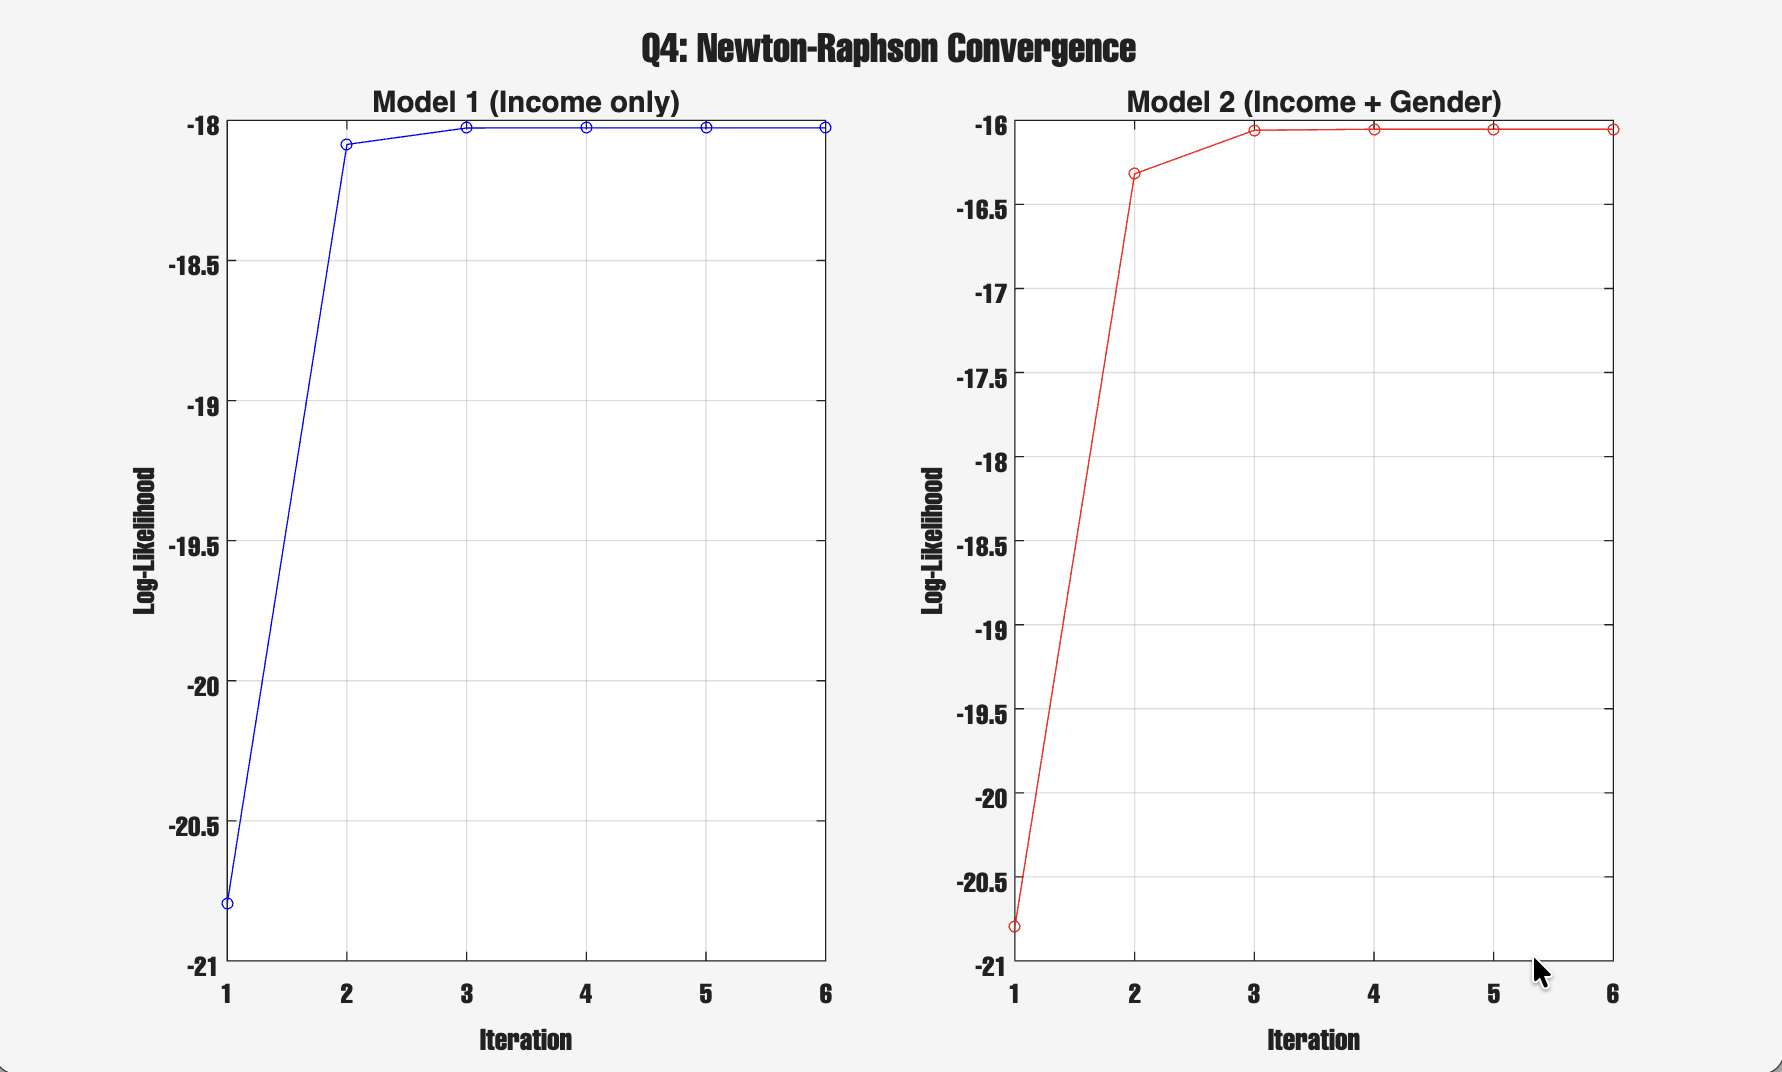
\includegraphics[width=0.90\textwidth]{../output/graph4.png}
\caption{Newton-Raphson log-likelihood convergence: Model~1 (left) and Model~2 (right)}
\end{figure}

\subsection{(c) JMP Validation}

Both models were re-estimated in JMP Student Edition (Analyze $\to$ Fit Model,
Personality: Nominal Logistic; Income set as Continuous, Gender set as Nominal).

\begin{figure}[H]
\centering
\begin{subfigure}[t]{0.48\textwidth}
  \centering
  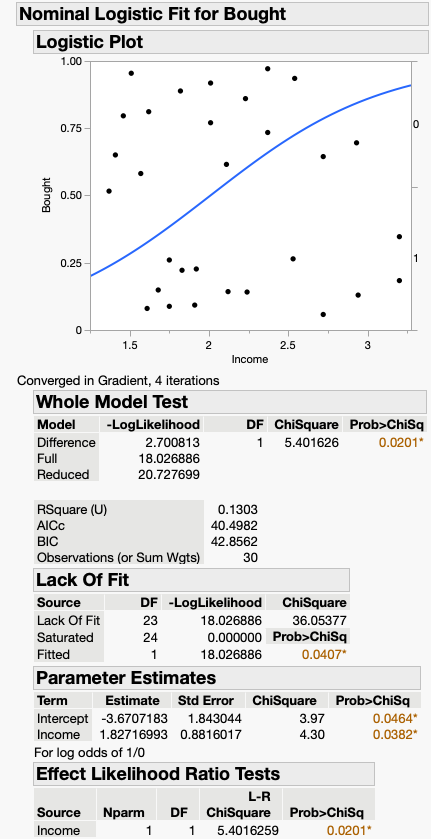
\includegraphics[width=\textwidth]{../output/JMP-q4c-model1.png}
  \caption{Model 1 (Income only)}
\end{subfigure}
\hfill
\begin{subfigure}[t]{0.48\textwidth}
  \centering
  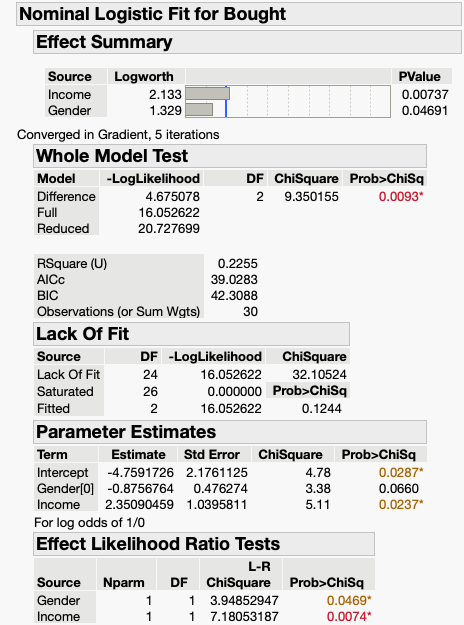
\includegraphics[width=\textwidth]{../output/JMP-q4c-model2.png}
  \caption{Model 2 (Income + Gender)}
\end{subfigure}
\caption{JMP Nominal Logistic Fit for Q4: Parameter Estimates, Whole Model Test,
and Effect Likelihood Ratio Tests.}
\end{figure}

\begin{table}[H]
\centering
\caption{Q4 Model 1 (Income only) coefficient comparison: MATLAB vs.\ JMP}
\begin{tabular}{lrrl}
\toprule
Parameter & MATLAB & JMP & Match? \\
\midrule
$\hat{b}_0$ (Intercept) & $-3.6707$ & $-3.6707$ & \checkmark \\
$\hat{b}_1$ (Income)    & $1.8272$  & $1.8272$  & \checkmark \\
Log-likelihood          & $-18.0269$ & $-18.0269$ & \checkmark \\
\bottomrule
\end{tabular}
\end{table}

\begin{table}[H]
\centering
\caption{Q4 Model 2 (Income + Gender) coefficient comparison: MATLAB vs.\ JMP}
\begin{tabular}{lrrl}
\toprule
Parameter & MATLAB (dummy coding) & JMP (effect coding) & Equivalent? \\
\midrule
$\hat{b}_0$ (Intercept) & $-5.6348$ & $-4.7592$ & \checkmark\textsuperscript{*} \\
$\hat{b}_1$ (Income)    & $2.3509$  & $2.3509$  & \checkmark \\
$\hat{b}_2$ (Gender)    & $1.7514$  & $2\times0.8757=1.7514$ & \checkmark\textsuperscript{*} \\
Log-likelihood          & $-16.0526$ & $-16.0526$ & \checkmark \\
\bottomrule
\end{tabular}
\end{table}

\noindent\textsuperscript{*}JMP uses \emph{effect coding} for the nominal Gender variable
(Gender[0] $= -0.8757$, Gender[1] $= +0.8757$), whereas MATLAB uses dummy coding
(Gender $= 0$ as reference). The two parameterisations are algebraically equivalent:
JMP's intercept $-4.7592$ plus the female effect $(-0.8757)$ equals the MATLAB intercept
$-5.6349 \approx -5.6348$; the male-vs-female log-odds difference $2 \times 0.8757 = 1.7514$
matches MATLAB's $\hat{b}_2$ exactly.
Income coefficient and log-likelihoods agree to 4 significant figures in both models.
Results verified against JMP Student Edition.

\clearpage
% ================================================================
\section{Question 5: Grouped Binomial MLE: Coupon Redemption}
% ================================================================

Grouped binomial data ($J = 5$ groups, $n_j = 200$ each):

\begin{table}[H]
\centering
\caption{Grouped binomial data: coupon redemption}
\begin{tabular}{rrrr}
\toprule
Price reduction $X_j$ (\$) & $n_j$ & $Y_j$ & Obs.\ $\hat{p}_j$ \\
\midrule
 5 & 200 &  30 & 0.1500 \\
10 & 200 &  55 & 0.2750 \\
15 & 200 &  70 & 0.3500 \\
20 & 200 & 100 & 0.5000 \\
30 & 200 & 137 & 0.6850 \\
\bottomrule
\end{tabular}
\end{table}

\subsection{Newton-Raphson Iterations}

\begin{table}[H]
\centering
\caption{Newton-Raphson iterations: Binomial MLE}
\begin{tabular}{crrr}
\toprule
Iteration & $\hat{b}_0$ & $\hat{b}_1$ & Log-likelihood \\
\midrule
1 & $-1.805405$ & 0.085838 & $-693.147181$ \\
2 & $-2.035627$ & 0.096437 & $-597.123859$ \\
3 & $-2.044336$ & 0.096833 & $-595.987828$ \\
4 & $-2.044348$ & 0.096834 & $-595.986344$ \\
5 & $-2.044348$ & 0.096834 & $-595.986344$ \\
\bottomrule
\end{tabular}
\end{table}

Converged at iteration 5.

\subsection{Estimated Parameters}

\begin{table}[H]
\centering
\caption{Binomial MLE: estimated parameters}
\begin{tabular}{lrrr}
\toprule
Parameter & Estimate & Std.\ Error & $z$-statistic \\
\midrule
$b_0$ (intercept)       & $-2.0443$ & 0.1610 & $-12.6996$ \\
$b_1$ (price reduction) &  0.0968   & 0.0085 &  11.3266   \\
\midrule
\multicolumn{3}{l}{Final log-likelihood} & $-595.9863$ \\
\bottomrule
\end{tabular}
\end{table}

\subsection{Predicted vs.\ Observed Proportions}

\begin{table}[H]
\centering
\caption{Predicted vs.\ observed proportions and deviance residuals}
\begin{tabular}{ccrrrr}
\toprule
$X_j$ & $n_j$ & $Y_j$ & Obs.\ $\hat{p}_j$ & Pred.\ $\hat{\pi}_j$ & Dev.\ residual \\
\midrule
 5 & 200 &  30 & 0.1500 & 0.1736 & $-0.8988$ \\
10 & 200 &  55 & 0.2750 & 0.2543 &  0.6678  \\
15 & 200 &  70 & 0.3500 & 0.3562 & $-0.1837$ \\
20 & 200 & 100 & 0.5000 & 0.4731 &  0.7612  \\
30 & 200 & 137 & 0.6850 & 0.7028 & $-0.5477$ \\
\bottomrule
\end{tabular}
\end{table}

\subsection{Goodness-of-Fit}

\[
  \chi^2_{\text{Pearson}} = 2.1486, \quad df = 3, \quad p\text{-value} = 0.5421
\]

The large $p$-value indicates no significant lack of fit; the logistic model provides
an adequate fit to the grouped data.

\subsection{Plots}

\begin{figure}[H]
\centering
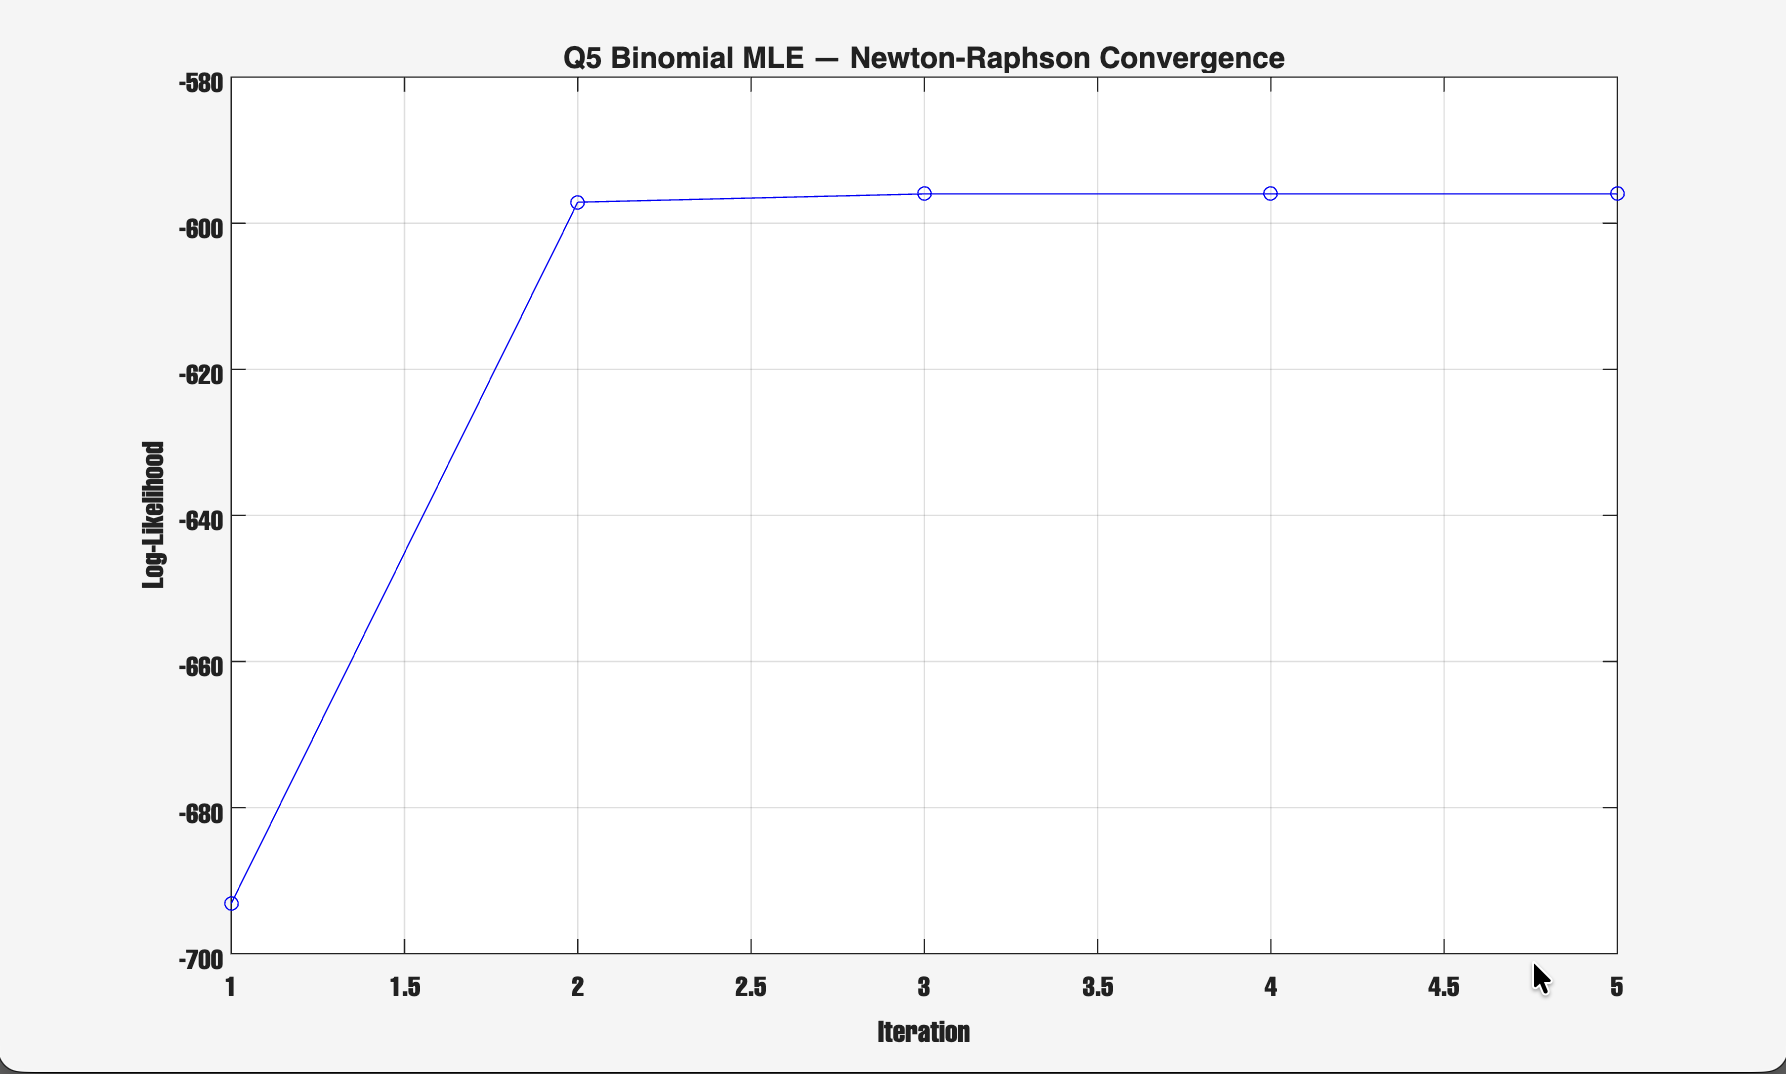
\includegraphics[width=0.80\textwidth]{../output/graph5-1.png}
\caption{Newton-Raphson log-likelihood convergence: Binomial MLE (Q5)}
\end{figure}

\begin{figure}[H]
\centering
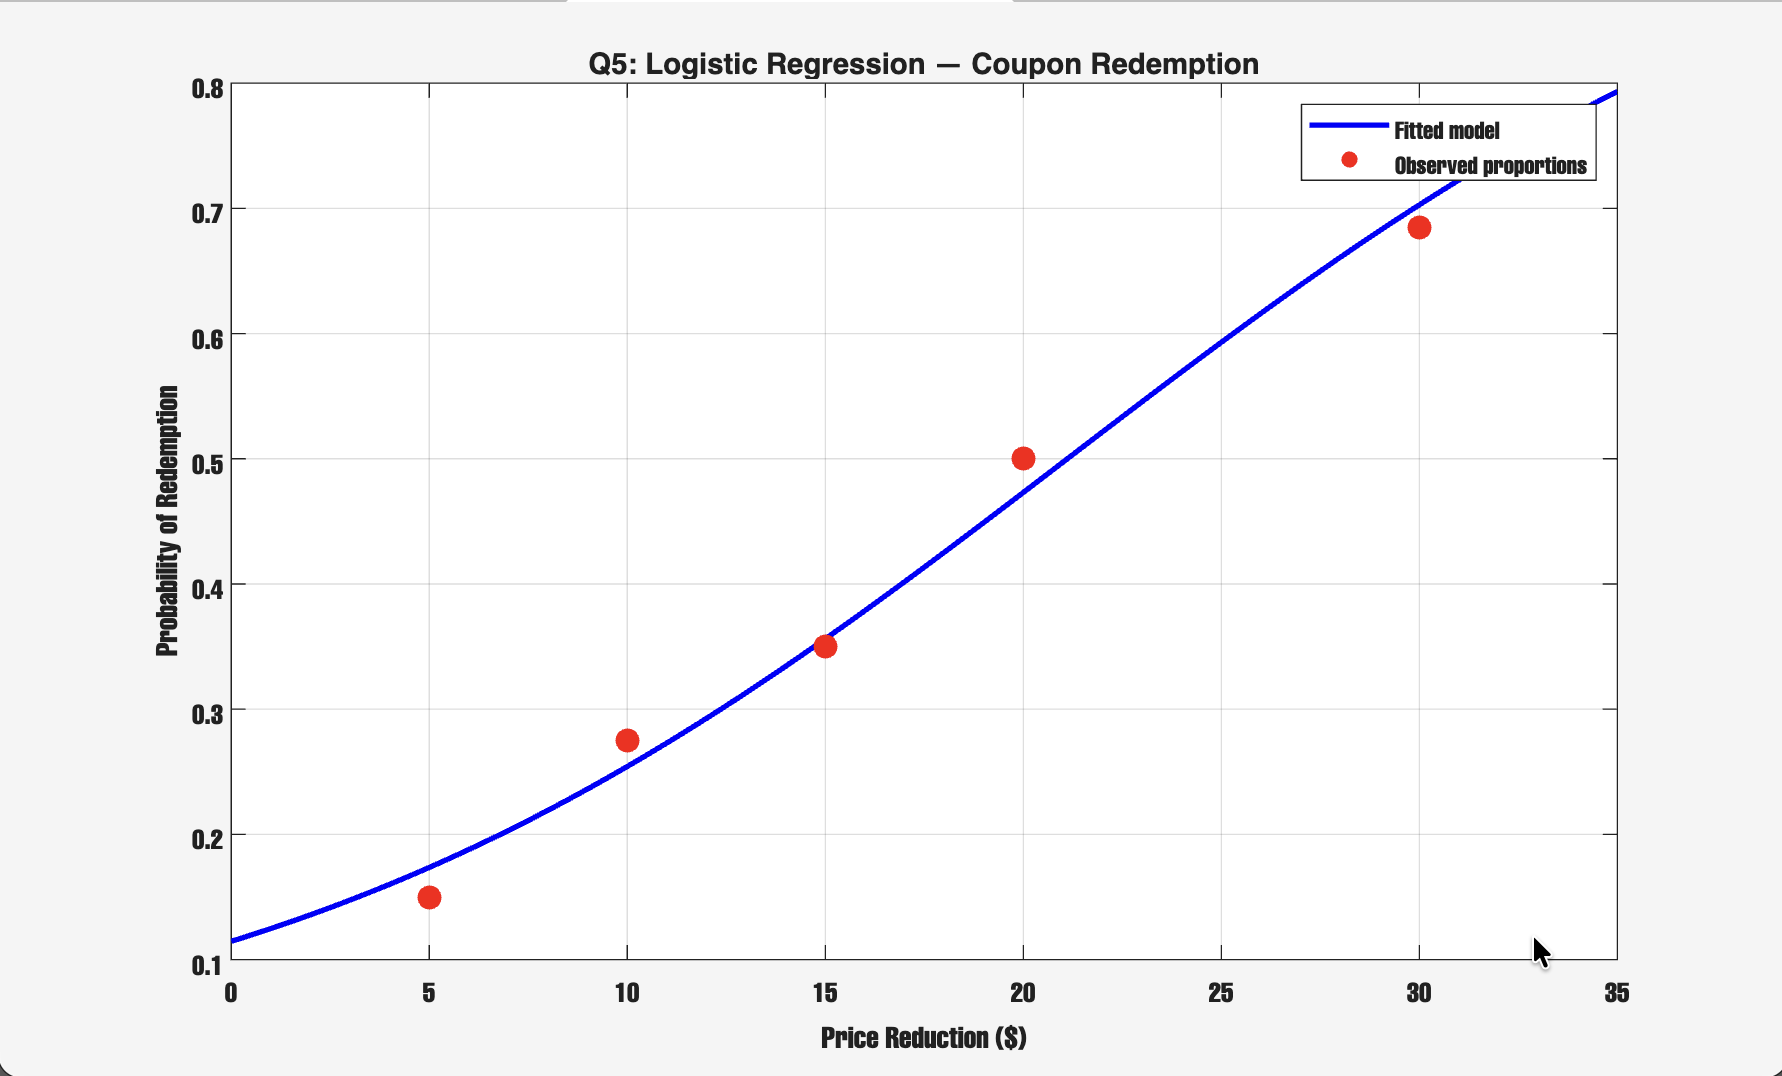
\includegraphics[width=0.80\textwidth]{../output/graph5-2.png}
\caption{Fitted logistic curve vs.\ observed proportions: Coupon redemption vs.\ price reduction}
\end{figure}

\clearpage
% ================================================================
\section{Question 6: Bernoulli MLE vs.\ Grouped Binomial}
% ================================================================

Data: $n = 30$ individual-level observations (16 with $y = 1$, 14 with $y = 0$).

\subsection{Newton-Raphson Iterations: Bernoulli MLE}

\begin{table}[H]
\centering
\caption{Newton-Raphson iterations: Bernoulli (ungrouped) MLE}
\begin{tabular}{crrr}
\toprule
Iteration & $\hat{b}_0$ & $\hat{b}_1$ & Log-likelihood \\
\midrule
1 & $-3.190626$ & 1.571513 & $-20.794415$ \\
2 & $-3.412405$ & 1.688309 & $-18.738363$ \\
3 & $-3.416112$ & 1.690360 & $-18.727749$ \\
4 & $-3.416114$ & 1.690361 & $-18.727745$ \\
5 & $-3.416114$ & 1.690361 & $-18.727745$ \\
\bottomrule
\end{tabular}
\end{table}

Converged at iteration 5.

\subsection{Estimated Parameters}

\begin{table}[H]
\centering
\caption{Bernoulli MLE: estimated parameters}
\begin{tabular}{lrr}
\toprule
Parameter & Estimate & Std.\ Error \\
\midrule
$b_0$ (intercept) & $-3.4161$ & 1.8918 \\
$b_1$ (Income)    &  1.6904   & 0.8893 \\
\midrule
\multicolumn{2}{l}{Final log-likelihood} & $-18.7277$ \\
\bottomrule
\end{tabular}
\end{table}

\subsection{Predicted vs.\ Observed (by Income Group)}

\begin{table}[H]
\centering
\caption{Predicted vs.\ observed proportions by income group}
\begin{tabular}{rrr}
\toprule
Group mean income & Obs.\ proportion & Pred.\ $\hat{\pi}$ \\
\midrule
2.7170 & 0.6667 & 0.7643 \\
2.5620 & 0.8333 & 0.7139 \\
2.0200 & 0.5000 & 0.4996 \\
1.7200 & 0.3333 & 0.3755 \\
1.5567 & 0.3333 & 0.3133 \\
\bottomrule
\end{tabular}
\end{table}

\subsection{Comparison: Bernoulli vs.\ Grouped Binomial}

\begin{table}[H]
\centering
\caption{Parameter estimates and standard errors: Bernoulli (Q6) vs.\ Grouped Binomial}
\begin{tabular}{lrrr}
\toprule
Parameter & Bernoulli & Grouped Binomial & Difference \\
\midrule
$b_0$ (intercept) & $-3.416114$ & $-3.416114$ & $4.4\times10^{-16}$ \\
$b_1$ (income)    &  1.690361   &  1.690361   & $2.2\times10^{-16}$ \\
\midrule
SE$(b_0)$         &  1.8918     &  1.8918     & 0 \\
SE$(b_1)$         &  0.8893     &  0.8893     & 0 \\
\bottomrule
\end{tabular}
\end{table}

\textbf{Interpretation.}\ Point estimates and standard errors are \emph{identical} (to
machine precision) because the sufficient statistic $X'y$ is the same for both
likelihoods when each individual's predictor equals the group mean. Standard errors
would differ only if individuals within a group had distinct predictor values, making
the Bernoulli and Binomial Fisher information matrices algebraically unequal.

\subsection{Newton-Raphson Convergence}

\begin{figure}[H]
\centering
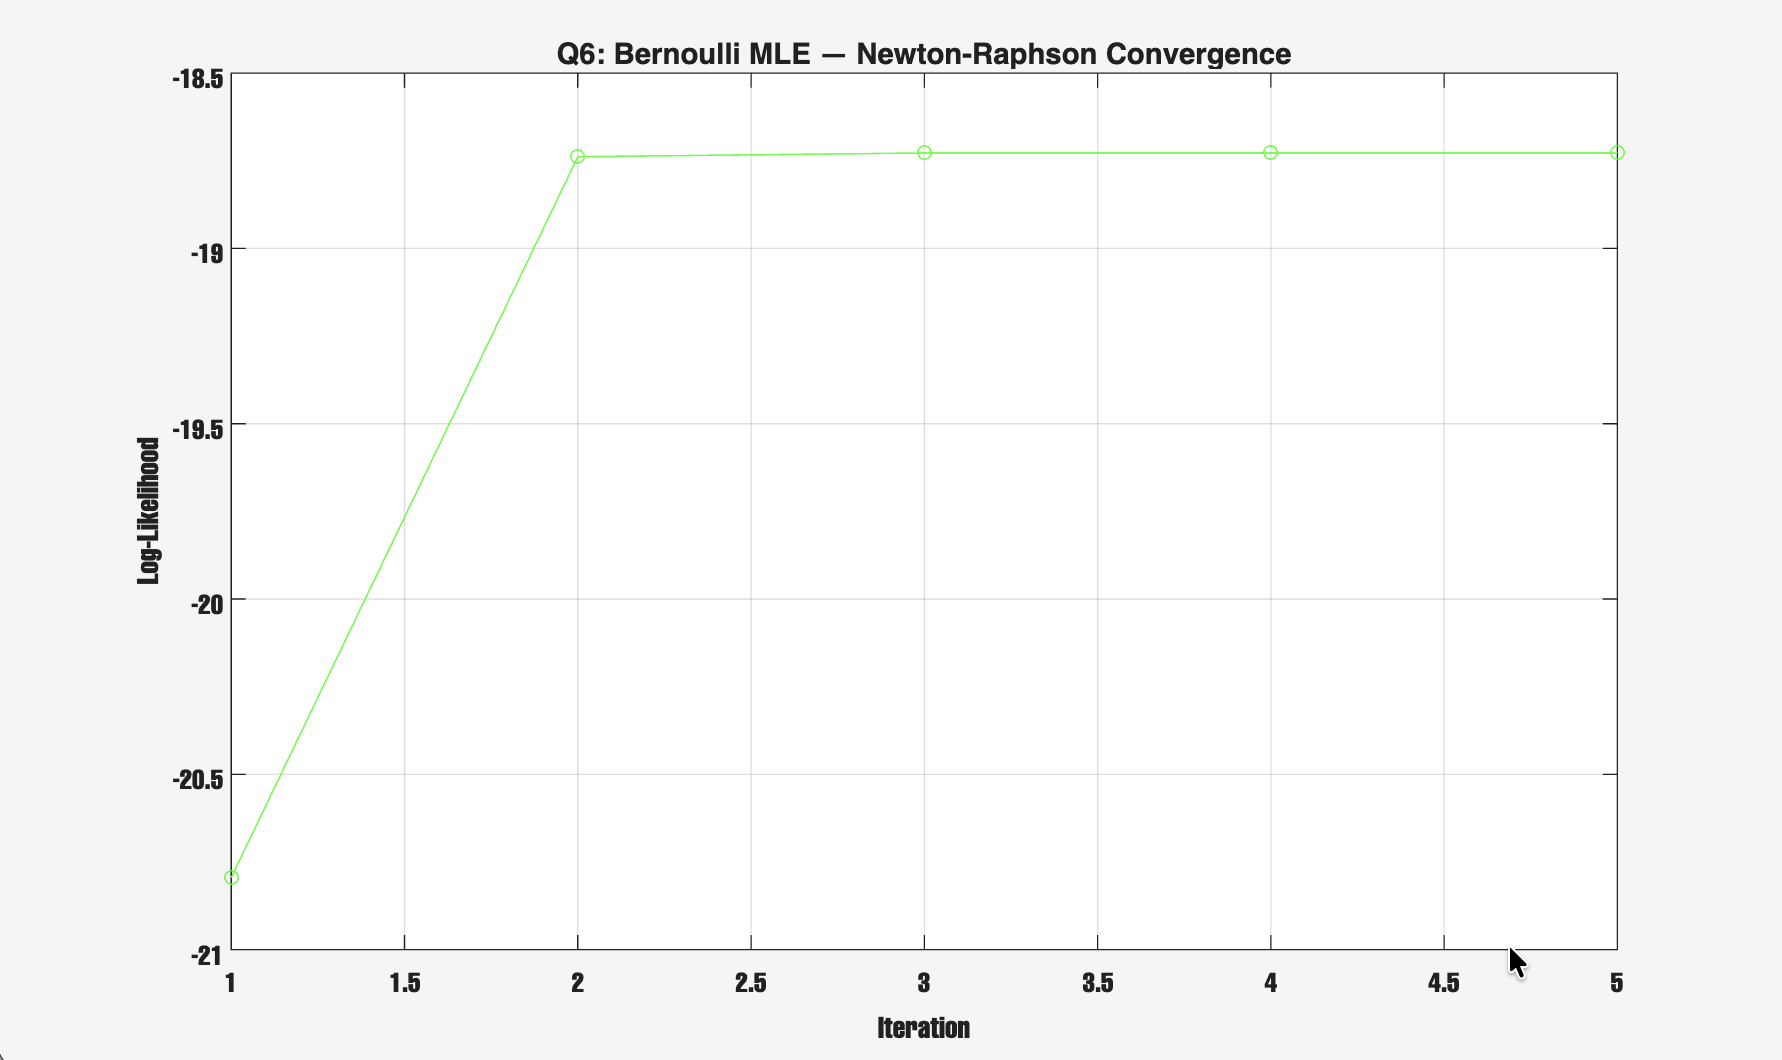
\includegraphics[width=0.80\textwidth]{../output/graph6.png}
\caption{Newton-Raphson log-likelihood convergence: Bernoulli MLE (Q6)}
\end{figure}

\clearpage
% ================================================================
\section{Question 7: Multiple Logistic Regression: Dengue Disease (Kutner CH14)}
% ================================================================

\subsection{Data Summary}

\begin{itemize}
  \item Dataset: Kutner CH14TA03, $n = 98$ individuals
  \item Disease ($Y = 1$): 31; No disease ($Y = 0$): 67
  \item Sector~1: 59 individuals; Sector~2: 39 individuals
  \item Upper SES (reference): 38; Middle SES: 24; Lower SES: 36
\end{itemize}

\textbf{Model: }
\[
  \text{logit}(\pi_i) = b_0
    + b_1 \cdot \text{Age}
    + b_2 \cdot \text{SES}_{\text{mid}}
    + b_3 \cdot \text{SES}_{\text{low}}
    + b_4 \cdot \text{Sector}
\]

where $\text{SES}_{\text{mid}}$ and $\text{SES}_{\text{low}}$ are dummy variables with
upper SES as the reference category, and Sector $= 1$ for Sector~2.

\subsection{Newton-Raphson Iterations}

\begin{table}[H]
\centering
\caption{Newton-Raphson iterations: Dengue disease model}
\footnotesize
\begin{tabular}{crrrrrrr}
\toprule
Iter & $b_0$ & $b_1$(Age) & $b_2$(mid) & $b_3$(low) & $b_4$(sec) & Log-lik \\
\midrule
1 & $-1.8120$ & 0.0222 &  0.3038 & $-0.1660$ & 1.2681 & $-67.9284$ \\
2 & $-2.2520$ & 0.0287 &  0.3959 & $-0.2801$ & 1.5374 & $-51.2093$ \\
3 & $-2.3118$ & 0.0297 &  0.4086 & $-0.3046$ & 1.5741 & $-50.5378$ \\
4 & $-2.3129$ & 0.0298 &  0.4088 & $-0.3053$ & 1.5747 & $-50.5271$ \\
5 & $-2.3129$ & 0.0298 &  0.4088 & $-0.3053$ & 1.5747 & $-50.5271$ \\
\bottomrule
\end{tabular}
\end{table}

Converged at iteration 6.

\subsection{Estimated Model Parameters}

\begin{table}[H]
\centering
\caption{Multiple logistic regression: parameter estimates, Dengue disease}
\begin{tabular}{lrrrr}
\toprule
Parameter & Estimate & Std.\ Error & $z$-stat & Odds Ratio \\
\midrule
$b_0$ (intercept)   & $-2.3129$ & 0.6426 & $-3.5994$ & 0.0990 \\
$b_1$ (Age)         &  0.0298   & 0.0135 &  2.2032   & 1.0302 \\
$b_2$ (SES mid)     &  0.4088   & 0.5990 &  0.6824   & 1.5050 \\
$b_3$ (SES low)     & $-0.3053$ & 0.6041 & $-0.5053$ & 0.7369 \\
$b_4$ (Sector~2)    &  1.5747   & 0.5016 &  3.1393   & 4.8295 \\
\midrule
\multicolumn{3}{l}{Final log-likelihood} & \multicolumn{2}{r}{$-50.5271$} \\
\bottomrule
\end{tabular}
\end{table}

\subsection{Predicted Probabilities (First 20 Observations)}

\begin{table}[H]
\centering
\caption{Predicted probabilities: first 20 of 98 observations}
\footnotesize
\begin{tabular}{cccccccc}
\toprule
Obs & $Y$ & Age & SES\,mid & SES\,low & Sector & $\hat{\pi}$ & Pred \\
\midrule
 1 & 0 & 33 & 0 & 0 & 0 & 0.2090 & 0 \\
 2 & 0 & 35 & 0 & 0 & 0 & 0.2190 & 0 \\
 3 & 0 &  6 & 0 & 0 & 0 & 0.1058 & 0 \\
 4 & 0 & 60 & 0 & 0 & 0 & 0.3710 & 0 \\
 5 & 1 & 18 & 0 & 1 & 0 & 0.1108 & 0 \\
 6 & 0 & 26 & 0 & 1 & 0 & 0.1365 & 0 \\
 7 & 0 &  6 & 0 & 1 & 0 & 0.0802 & 0 \\
 8 & 1 & 31 & 1 & 0 & 0 & 0.2725 & 0 \\
 9 & 1 & 26 & 1 & 0 & 0 & 0.2440 & 0 \\
10 & 0 & 37 & 1 & 0 & 0 & 0.3093 & 0 \\
11 & 0 & 23 & 0 & 0 & 0 & 0.1640 & 0 \\
12 & 0 & 23 & 0 & 0 & 0 & 0.1640 & 0 \\
13 & 0 & 27 & 0 & 0 & 0 & 0.1810 & 0 \\
14 & 1 &  9 & 0 & 0 & 0 & 0.1145 & 0 \\
15 & 1 & 37 & 0 & 0 & 1 & 0.5897 & 1 \\
16 & 1 & 22 & 0 & 0 & 1 & 0.4791 & 0 \\
17 & 1 & 67 & 0 & 0 & 1 & 0.7782 & 1 \\
18 & 0 &  8 & 0 & 0 & 1 & 0.3775 & 0 \\
19 & 1 &  6 & 0 & 0 & 1 & 0.3636 & 0 \\
20 & 1 & 15 & 0 & 0 & 1 & 0.4275 & 0 \\
\bottomrule
\multicolumn{8}{l}{\footnotesize (Showing first 20 of 98 observations)}
\end{tabular}
\end{table}

Classification accuracy (threshold 0.5): \textbf{71.4\%}.

\subsection{Model Significance (Likelihood Ratio Test vs.\ Null)}

\[
  G^2 = 2\,(\ell_{\text{full}} - \ell_{\text{null}})
       = 2\,(-50.5271 - (-61.1588))
       = 21.2635, \quad df = 4, \quad p\text{-value} = 0.000281
\]

The model is highly statistically significant: the four predictors (Age, SES, Sector)
jointly explain a significant portion of the variability in disease status.

\subsection{Interpretation}

\begin{itemize}
  \item \textbf{Age} ($b_1 = 0.0298 > 0$, OR $= 1.03$): Each additional year of age
        increases the odds of disease by $\sim 3\%$. Statistically significant
        ($z = 2.20$).
  \item \textbf{SES mid} ($b_2 = 0.4088 > 0$, OR $= 1.51$): Middle SES has
        $1.5\times$ higher disease odds than upper SES, but this effect is not
        statistically significant ($z = 0.68$).
  \item \textbf{SES low} ($b_3 = -0.3053 < 0$, OR $= 0.74$): Lower SES shows slightly
        lower odds than upper SES after adjusting for age and sector, not significant
        ($z = -0.51$). The direction of the SES low coefficient should be verified
        against the textbook column mapping.
  \item \textbf{Sector~2} ($b_4 = 1.5747 > 0$, OR $= 4.83$): The dominant predictor.
        Residents of Sector~2 have nearly \textbf{five times} the disease odds of
        Sector~1 residents, after adjusting for age and SES. Highly significant
        ($z = 3.14$).
\end{itemize}

\subsection{Newton-Raphson Convergence}

\begin{figure}[H]
\centering
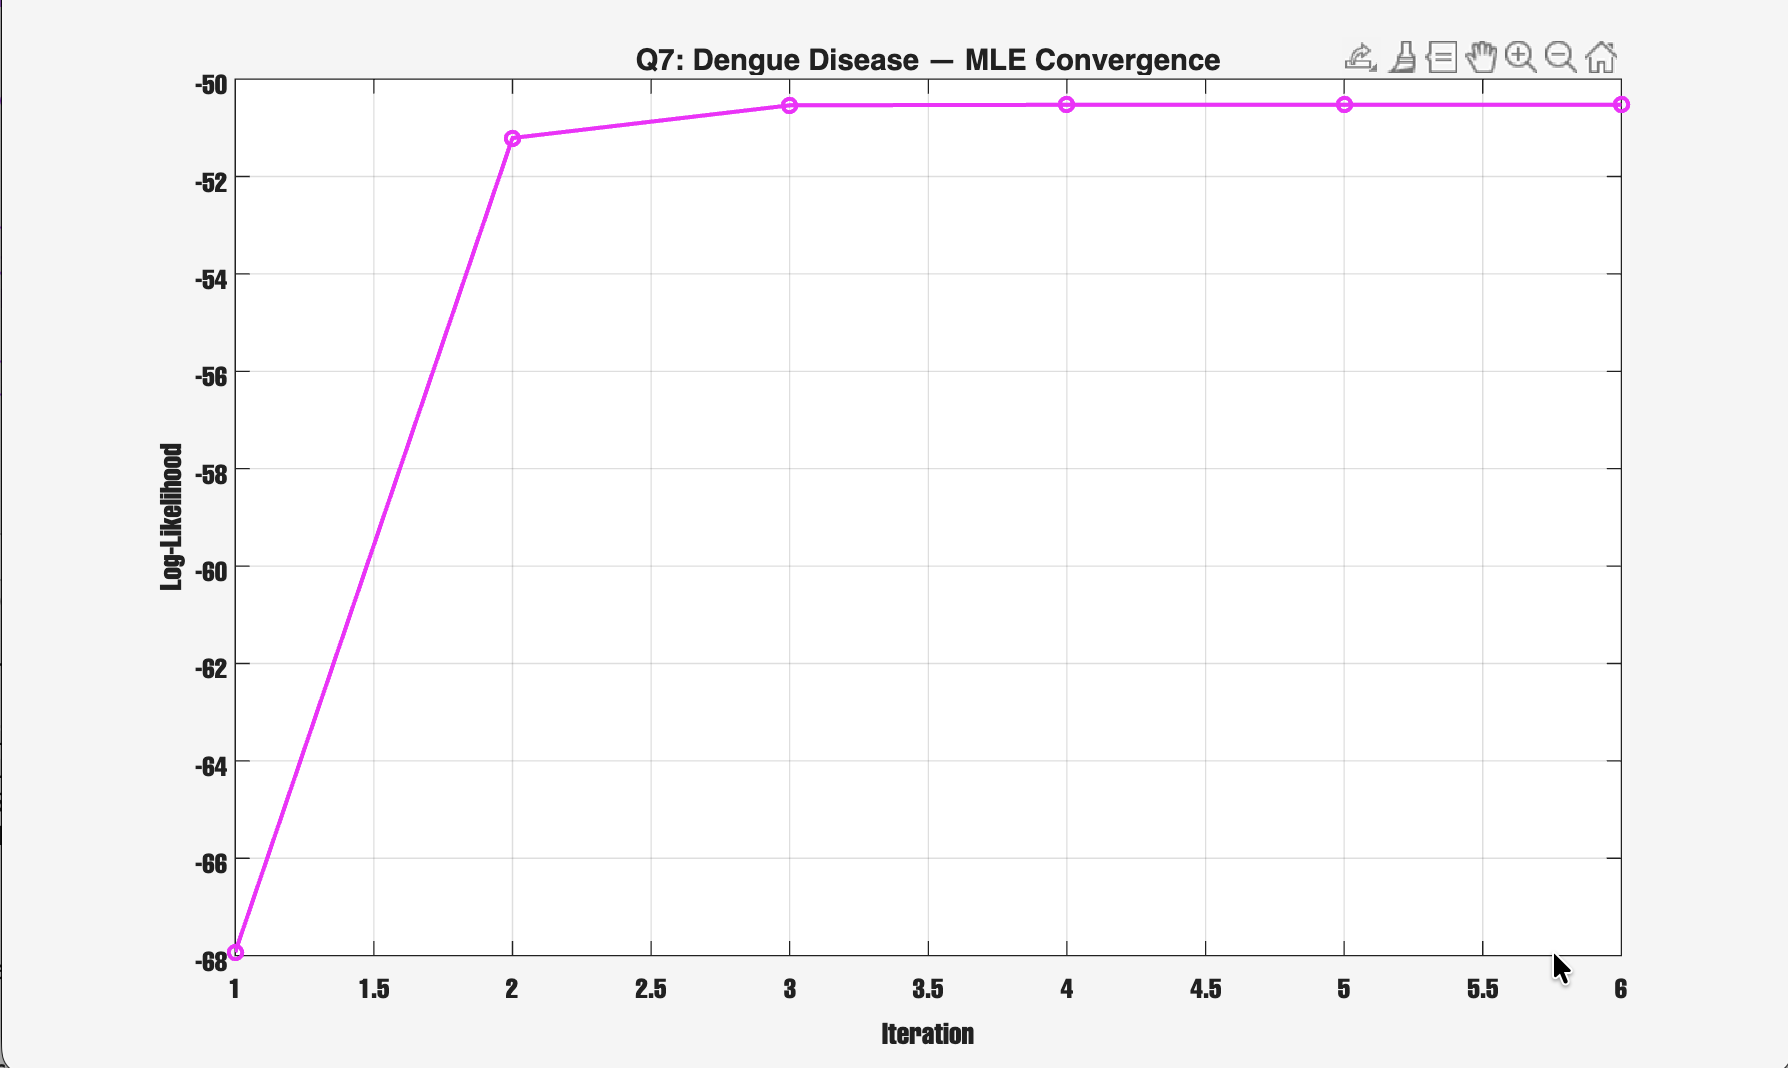
\includegraphics[width=0.80\textwidth]{../output/graph7.png}
\caption{Newton-Raphson log-likelihood convergence: Dengue disease model (Q7)}
\end{figure}

\end{document}
